\documentclass[a4paper, 11pt]{article}
\usepackage[utf8]{inputenc}
\usepackage[T1]{fontenc}

\usepackage[margin=1in]{geometry}
\usepackage{amsmath, amsfonts, amsthm, amssymb, amsxtra}

\usepackage{graphicx}
\usepackage{float}

\usepackage[dvipsnames]{xcolor}

\usepackage{tabularray}
\usepackage{enumitem}
\usepackage{multicol}

\usepackage{hyperref}
\hypersetup{hidelinks}

\usepackage{tikz}
\usetikzlibrary{intersections, angles, calc, positioning}
\usetikzlibrary{shapes.geometric, arrows.meta}
\usetikzlibrary{decorations.pathmorphing, decorations.pathreplacing}

\usepackage{minted}

\setlength{\parindent}{0pt}
\setlength{\parskip}{5pt}

\makeatletter
\newcommand{\type}[1]{\def\@type{#1}}

\renewcommand*{\maketitle}{%
\vspace{-0.5cm}
\begin{tikzpicture}[remember picture, overlay]
    \node[anchor=south, align=center] (date) at ($(current page.north) + (0,-110pt)$) {\@date};
    \node[anchor=south, align=center, font=\itshape] (author) at (date.north) {\@author};
    \node[above=10pt of author, align=center, font=\scshape] (type) {\@type};
    \node[anchor=south, align=center, font=\bfseries\large] (title) at (type.north) {\@title};
    \node[anchor=west] (logo) at ($(current page.north west) + (\Gm@lmargin, -65pt)$) {
\includegraphics[height=3.15cm]{figures/ufs_vertical_positiva.eps}};
    \draw ($(current page.north west) + (\Gm@lmargin, -120pt)$) -- ($(current page.north east) + (-\Gm@lmargin, -120pt)$);
\end{tikzpicture}
\vspace{35pt}
}%
\makeatother

\usepackage{notomath}

\definecolor{azulfundo}{RGB}{51, 149, 255}
\definecolor{cinzaborda}{RGB}{66, 73, 80}
\definecolor{bicoum}{RGB}{181, 141, 57}
\definecolor{bicodois}{RGB}{206, 157, 56}
\definecolor{novo}{RGB}{108, 107, 91}

\title{EFEITO BLUR EM\\IMAGENS .ppm}
\type{Atividade}
\author{Bruno Sant'Anna}
\date{\today}

\begin{document}
\maketitle

\section*{Introdução}
Uma \textit{convolução} é uma operação matemática com muitas utilidades, inclusive em computação gráfica e processamento de imagens.
Por meio de um \textit{kernel de convolução}, que é uma matriz pequena com uma série de pesos, que mudam o valor de um pixel na imagem dependendo dos valores dos pixels ao seu redor.
Nesse caso para aplicar um efeito de \textit{blur}, estaremos usando um kernel onde a soma de todos os pesos é igual a 1, por exemplo
\begin{equation}\label{eq:uniform}
    \begin{pmatrix}
        \frac{1}{9} & \frac{1}{9} & \frac{1}{9}\\[5pt]
        \frac{1}{9} & \frac{1}{9} & \frac{1}{9}\\[5pt]
        \frac{1}{9} & \frac{1}{9} & \frac{1}{9}
    \end{pmatrix}
\end{equation}

\begin{equation}\label{eq:gaussian}
    \begin{pmatrix}
        0.003 & 0.013 & 0.022 & 0.013 & 0.003\\
        0.013 & 0.060 & 0.098 & 0.060 & 0.013\\
        0.022 & 0.098 & 0.162 & 0.098 & 0.022\\
        0.013 & 0.060 & 0.098 & 0.060 & 0.013\\
        0.003 & 0.013 & 0.022 & 0.013 & 0.003
    \end{pmatrix}
\end{equation}
a matriz \ref{eq:uniform} aplica um blur uniforme, fazendo uma media aritmética dos pontos ao redor do centro, já a matriz \ref*{eq:gaussian} segue a distribuição gaussiana e aplica um peso maior ao centro.

\vspace{-0.5cm}
\section*{Funcionamento}

De forma simplificada, quando aplicamos um kernel em uma imagem, para cada pixel $(i,j)$ da imagem o kernel é posicionado com o seu centro em $(i,j)$ e multiplicamos o cada coordenada da imagem com a coordenada do kernel sobreposto e somamos, esse é o valor do pixel $(i,j)$ na imagem nova.
Vale lembrar que cada pixel da imagem colorida é um vetor de $\mathbf{N}^3$ onde cada entrada varia de 0 a 255, a primeira entrada é o canal de cor vermelho, a segunda verde e a terceira azul, conhecido como sistema RGB.

Usando o kernel \ref{eq:uniform} como exemplo:


\begin{center}
    \begin{minipage}{0.37\textwidth}
        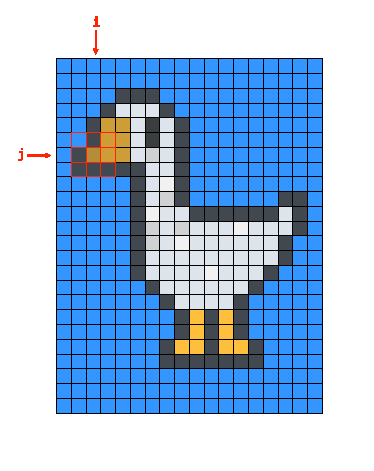
\includegraphics[height=7.25cm]{figures/goose.pdf}
    \end{minipage}
    \begin{minipage}{0.55\textwidth}
        $
        \left\lfloor
        \textcolor{azulfundo}{\frac{1}{9} \blacksquare} +
        \textcolor{cinzaborda}{\frac{1}{9} \blacksquare} +
        \textcolor{bicodois}{\frac{1}{9} \blacksquare} +
        \textcolor{cinzaborda}{\frac{1}{9} \blacksquare} + 
        \textcolor{bicoum}{\frac{1}{9} \blacksquare} + 
        \textcolor{bicodois}{\frac{1}{9} \blacksquare} +
        \textcolor{cinzaborda}{\frac{1}{9} \blacksquare} + 
        \textcolor{cinzaborda}{\frac{1}{9} \blacksquare} + 
        \textcolor{cinzaborda}{\frac{1}{9} \blacksquare}
        \right\rfloor  = \textcolor{novo}{\blacksquare}
        $
    \end{minipage}
\end{center}

Ou com a notação vetorial

$$
\left\lfloor
\frac{1}{9}
\begin{bmatrix}
    \textcolor{red}{51} \\ \textcolor{green}{149} \\ \textcolor{blue}{255}
\end{bmatrix}+
\frac{1}{9}
\begin{bmatrix}
    \textcolor{red}{66} \\ \textcolor{green}{73} \\ \textcolor{blue}{80}
\end{bmatrix} +
\frac{1}{9}
\begin{bmatrix}
    \textcolor{red}{206} \\ \textcolor{green}{157} \\ \textcolor{blue}{56}
\end{bmatrix} +
\frac{1}{9}
\begin{bmatrix}
    \textcolor{red}{66} \\ \textcolor{green}{73} \\ \textcolor{blue}{80}
\end{bmatrix} +
\frac{1}{9}
\begin{bmatrix}
    \textcolor{red}{181} \\ \textcolor{green}{141} \\ \textcolor{blue}{57}
\end{bmatrix} +
\begin{bmatrix}
    \textcolor{red}{206} \\ \textcolor{green}{157} \\ \textcolor{blue}{56}
\end{bmatrix} +
\frac{1}{9}
\begin{bmatrix}
    \textcolor{red}{66} \\ \textcolor{green}{73} \\ \textcolor{blue}{80}
\end{bmatrix} +
\frac{1}{9}
\begin{bmatrix}
    \textcolor{red}{66} \\ \textcolor{green}{73} \\ \textcolor{blue}{80}
\end{bmatrix} +
\frac{1}{9}
\begin{bmatrix}
    \textcolor{red}{66} \\ \textcolor{green}{73} \\ \textcolor{blue}{80}
\end{bmatrix}
\right\rfloor = 
\frac{1}{9}
\begin{bmatrix}
    \textcolor{red}{108} \\ \textcolor{green}{107} \\ \textcolor{blue}{91}
\end{bmatrix}
$$


\section*{Resultados}
\begin{center}
    
\includegraphics[height=4cm]{figures/goose.png} \raisebox{2cm}{$\to$} 
\includegraphics[height=4cm]{figures/goose_blur.png}
\end{center}
\begin{center}
    \begin{tblr}{
        colspec={cc},
        row{2,4,6} = {font=\tiny},
        row{1,3,5} = {belowsep=1pt}
        }
        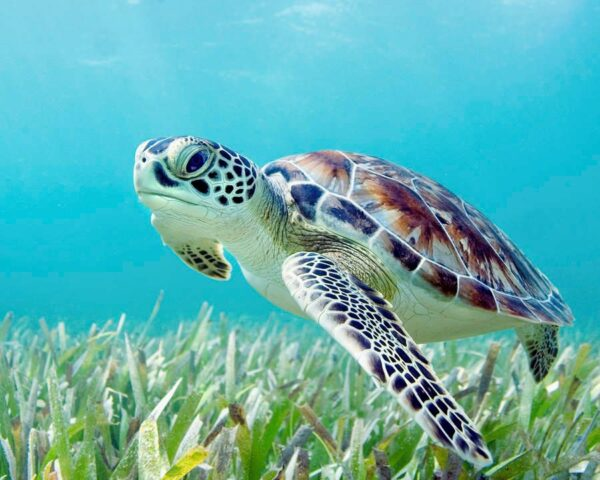
\includegraphics[width=5cm]{figures/turtle.png} & 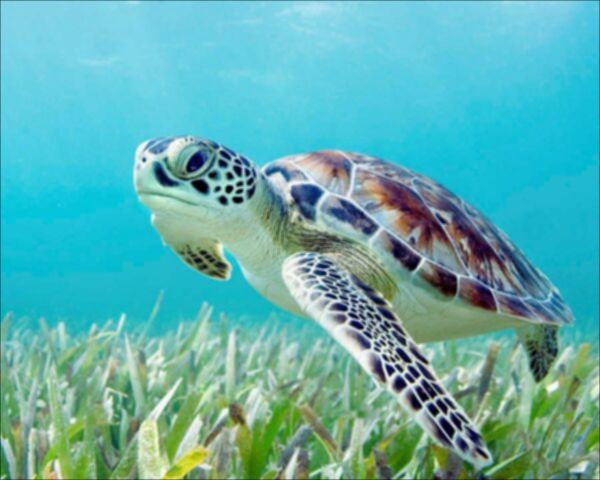
\includegraphics[width=5cm]{figures/turtle3x3.png} \\
        Imagem original & Blur com kernel uniforme $3 \times 3$ (eq. \ref{eq:uniform}) \\[2pt]
        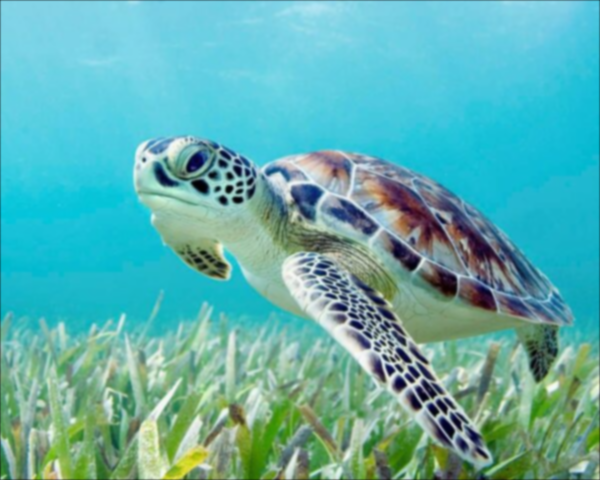
\includegraphics[width=5cm]{figures/turtle5x5.png} & 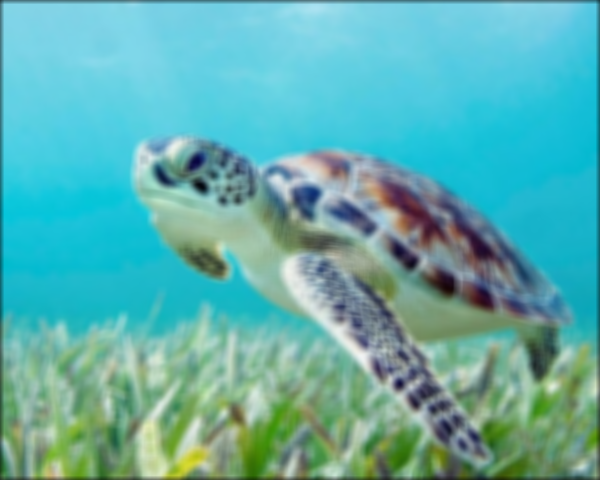
\includegraphics[width=5cm]{figures/turtle9x9.png} \\
        Blur com kernel gaussiano $5 \times 5$ (eq. \ref{eq:gaussian}) & Blur com kernel uniforme $9 \times 9$ \\[2pt]
        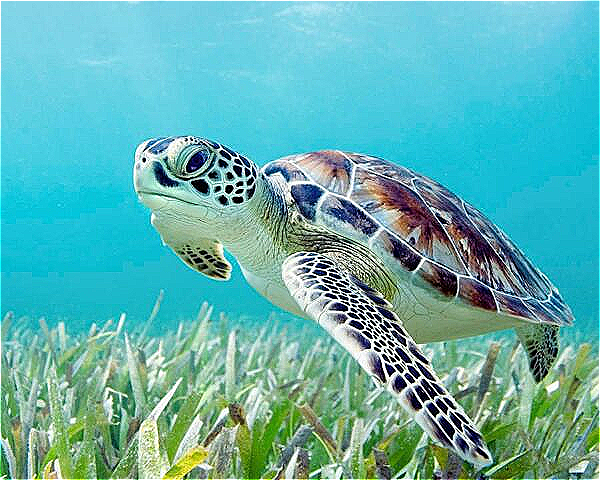
\includegraphics[width=5cm]{figures/turtle_sharpen.png} & 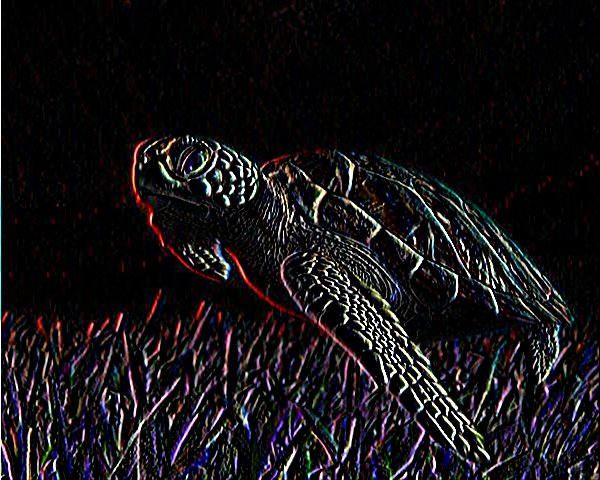
\includegraphics[width=5cm]{figures/turtle_edge.png} \\
        Aumento de nitidez (\textit{sharpen}) $5 \times 5$ &  Detecção de borda
    \end{tblr}
\end{center}

Onde a matriz usada para o efeito \textit{sharpen} é
\begin{equation}
    \begin{pmatrix}
        0 & -1 & 0\\
        -1 & \:\:\:5 & -1\\
        0 & -1 & 0
    \end{pmatrix}
\end{equation}
e para detecção de bordas
\begin{equation}
    \begin{pmatrix}
        -1 & 0 & 1\\
        -2 & 0 & 2\\
        -1 & 0 & 1
    \end{pmatrix}
\end{equation}

\section*{Código fonte}
\begin{minted}[autogobble, mathescape, breaklines, linenos]{c}
    void conv(int height, int length, int width, int kernelSize, unsigned char (**A)[3], float (*B)[kernelSize], int y, int x, unsigned char *output){
        int i, j, k, I, J;

        float s[3] = {0,0,0};
        int m = floor(kernelSize*0.5);
        int n = kernelSize - m;
        for (i = y-m ; i < y+n; i++){
            for (j = x-m; j < x+n; j++){
                if (i >= 0 && i < height && j >= 0 && j < length){
                    I = i - (y-m);
                    J = j - (x-m);
                    s[0] += A[i][j][0] * B[I][J];
                    s[1] += A[i][j][1] * B[I][J];
                    s[2] += A[i][j][2] * B[I][J];
                }
            }
        }
        for (i = 0; i < 3; i++){
            output[i] = floor(s[i]);
        }
    }

    void main(){
        int i, j, k, l, h;
        unsigned char type, cmax, caractere;
        FILE *fp;

        // TROCAR NOME DO ARQUIVO AQUI
        fp = fopen("turtle.ppm", "r");
        while ((caractere=getc(fp))=='#')
            while((caractere=getc(fp))!='\n');
        ungetc(caractere,fp);

        fscanf(fp, "P%hhu\n", &type);
        while ((caractere=getc(fp))=='#')
            while((caractere=getc(fp))!='\n');
        ungetc(caractere,fp);

        fscanf(fp, "%u %u\n%hhu\n", &l, &h, &cmax);


        unsigned char (**imagem)[3];

        j=l*sizeof(char*);
        imagem = malloc(j);

        j=h*3;
        for (i=0; i<l; i++)
            imagem[i] = malloc(j);

        if(type==3){
            for(j=0; j<h; j++)
                for(i=0; i<l; i++)
                    fscanf(fp, "%hhu %hhu %hhu", &imagem[i][j][0],&imagem[i][j][1],&imagem[i][j][2]);
            fclose(fp);
        }
        else if(type==6){
            for(j=0; j<h; j++)
                for(i=0; i<l; i++)
                    fscanf(fp, "%c%c%c", &imagem[i][j][0],&imagem[i][j][1],&imagem[i][j][2]);
            fclose(fp);
        }       
        else{
            printf("Formato inválido!");
            fclose(fp);
            exit(0);
        }

        unsigned char (**blur)[3];
        j=h*sizeof(char*);
        blur = malloc(j);

        j=h*3;
        for (i=0; i<l; i++)
            blur[i] = malloc(j);

        unsigned char aux[3];

        // KERNEL DE CONVOLUÇÃO
        float uniform[5][5];
        for (i = 0; i < 5; i++){
            for (j = 0; j < 5; j++){
                uniform[i][j] = 0.04;
            }
        }

        double gaussian[5][5] = {
            {0.003, 0.013, 0.022, 0.013, 0.003},
            {0.013, 0.060, 0.098, 0.060, 0.013},
            {0.022, 0.098, 0.162, 0.098, 0.022},
            {0.013, 0.060, 0.098, 0.060, 0.013},
            {0.003, 0.013, 0.022, 0.013, 0.003}
        };

        int sharpen[3][3] = {
            {0, -1,  0},
            {-1, 5, -1},
            {0, -1,  0}
        };

        int bordas[3][3] = {
            {-1, 0, 1},
            {-2, 0, 2},
            {-1, 0, 1}
        };
        
        // APLICANDO O EFEITO DE BLUR
        for (j = 0; j < h; j++){
            for (i = 0; i < l; i++){
                conv(l,h,3,5,imagem,uniform,i,j,aux);
                blur[i][j][0] = aux[0];
                blur[i][j][1] = aux[1];
                blur[i][j][2] = aux[2];
            }
        }
        
        // EXPORTANDO A IMAGEM
        fp = fopen("blur.ppm", "w");
        fprintf(fp, "P6\n");
            fprintf(fp, "%u %u\n255\n", l, h);
            for (j=0;j<h;j++)
                for (i=0;i<l;i++)
                    fprintf(fp,"%c%c%c", blur[i][j][0],blur[i][j][1],blur[i][j][2]);
            fclose(fp);
    }
\end{minted} 
\end{document}